\chapter{Локализация источников гамма-всплесков методом триангуляции} \label{IPN_catalog}
\section{Введение}
Для каждого всплеска из набора 296 коротких гамма-всплесков, рассмотренного в 
предыдущей главе, был произведён поиск детектирования на КА, входящих в межпланетную 
сеть Interplanetary Network (IPN). Было обнаружено, что 271 ($\sim 92$\%) коротких 
всплесков Конус-Винд (KW) были зарегистрированы по крайней мере одним КА IPN, 
что позволило получить их локализацию триангуляционным методом.

В период с ноября 1994~г. по декабрь 2010~г. IPN содержала от 3-х до 11 КА. 
За все время существования IPN туда, помимо KW, входили следующие аппараты
на большом удалении от Земли: 
\begin{itemize}
\item \textit{Ulysses}, находившийся на гелиоцентрической орбите расстоянии 
670--3180 световых секунды от Земли, с инструментом для изучения рентгеновского 
излучения Солнца и гамма-всплесков GRB~\citep{Hurley_1992AAS};
\item \textit{Near-Earth Asteroid Rendezvous} (\textit{NEAR}), находившийся 
на расстоянии до 3100 световых секунд от Земли, с рентгеновским/гамма-спектрометром XGRS~\citep{Trombka_1999NIMPA};
\item \textit{Mars Odyssey}, запущенный в апреле 2001~г и достигший орбиты вокруг 
Марса в октябре 2001~г на расстоянии до 1250 световых секунд от Земли~\citep{Saunders_2004SSRv}, 
КА оборудован гамма-спектрометром GRS, в состав которого входят два детектора 
с возможностью регистрировать гамма-всплески: гамма-детектор GSH и детектор 
высокоэнергичных нейтронов HEND~\citep{Boynton_2004SSRv, Hurley_2006ApJS_MO};
\item \textit{Mercury Surface, Space Environment, Geochemistry, and Ranging} (\textit{MESSENGER}) 
со спектрометром гамма-излучения и нейтронов GRNS~\citep{Goldsten_2007SSRv}, 
запущенный в августе 2004~г и вышедший на орбиту вокруг Меркурия в марте 2011~г 
на расстоянии до 700 световых секунд от Земли, полное функционирование КА 
началось в 2007~г~\citep{Gold_2001PSS,Solomon_2007SSRv};
\item \textit{International Gamma-Ray Astrophysics Laboratory} (\textit{INTEGRAL}), 
где в качестве детектора гамма излучения выступает защита (ACS) спектрометра 
SPI (SPI-ACS)~\citep{Rau_2005AA}, КА находится на вытянутой орбите с максимальным 
удалением до 0.5 световых секунд от Земли;
\end{itemize}

на околоземных орбитах:
\begin{itemize}
\item \textit{Compton Gamma-Ray Observatory} (\textit{CGRO}) с экспериментом 
Burst and Transient Source Experiment (BATSE)~\citep{Fishman_1992NASCP3137};
\item \textit{BeppoSAX} с экспериментом Gamma-Ray Burst Monitor (GRBM)~\citep{Frontera_1997AAS,Feroci_1997SPIE};
\item \textit{Reuven Ramaty High Energy Solar Spectroscopic Imager} (\textit{RHESSI})~\citep{Lin_2002SoPh, Smith_2002SoPh};
\item \textit{High Energy Transient Explorer} (\textit{HETE-2}) с телескопом 
French Gamma-Ray Telescope (FREGATE)~\citep{Ricker_2003AIPC, Atteia_2003AIPC};
\item \textit{Swift} с телескопом Burst Alert Telescope (BAT)~\citep{Barthelmy_2005SSRv,Gehrels_2004ApJ};
\item \textit{Suzaku} с телескопом Wide-band All-sky Monitor (WAM)~\citep{Yamaoka_2009PASJ,Takahashi_2007PASJ};
\item \textit{AGILE} с инструментами Mini-Calorimeter (MCAL) и Super-AGILE~\citep{Tavani_2009AA};
\item \textit{Fermi} с иструментом Gamma-Ray Burst Monitor (GBM)~\citep{Meegan_2009ApJ};
\item Солнечная обсерватория \textit{Коронас-Ф} с гамма-спектрометром Геликон~\citep{Oraevskii_2002PhyU};
\item КА \textit{Космос~2326} с гамма-спектрометром Конус-А~\citep{Aptekar_1998ApJ};
\item КА \textit{Космос~2367} с гамма-спектрометром Конус-А2;
\item КА \textit{Космос~2421} с гамма-спектрометром Конус-А3 и
\item Солнечная обсерватория \textit{Коронас-Фотон} с гамма-спектрометром Конус-РФ.
\end{itemize}

По крайней мере два других КА наблюдали гамма-всплески в рассматриваемый период:
\textit{Defense Meteorological Satellite Program}
(\textit{DMSP})~\citep{Terrell_1998AIPC,Terrell_1996AIPC,Terrell_2004AIPC} и 
\textit{Stretched Rohini Satellite Series} (\textit{SROSS})~\citep{Marar_1994AA}.
Однако они не использовались для триангуляции, поэтому они не относятся к IPN. 

Далее представлена методика локализации и результаты, полученные для 271 короткого 
всплеска Конус-Винд, детектированных по крайней мере ещё одним КА IPN.

\section{Наблюдения}\label{sec:IPN_catalog_obserations}
Для каждого короткого всплеска Конус-Винд производился поиск в данных КА сети IPN. 
Для околоземных КА и \textit{INTEGRAL} временн\'{о}е окно поиска было центрировано 
на времени срабатывания триггера KW, ширина окна соответствовала расстоянию, 
немного превышающему расстояние от Земли до \textit{Wind}. Для КА в межпланетном 
пространстве ширина окна поиска соответствовала удвоенному расстоянию до КА, если 
направление прихода излучения было неизвестно, что имело место для большинства событий. 
Если направление прихода было известно хотя бы грубо, то вычислялось ожидаемое время 
прихода излучения на КА и производился поиск вблизи этого времени.

Временные интервалы существования различных КА в IPN и число коротких всплесков 
KW, зарегистрированных каждым КА/инструментом показаны на рис.~\ref{img:Mission_timeline}. 
Наибольшее число зарегистрированных всплесков 139, после KW, 
было зарегистрировано \textit{INTEGRAL}~(SPI-ACS).

\begin{figure}[h]
    \center{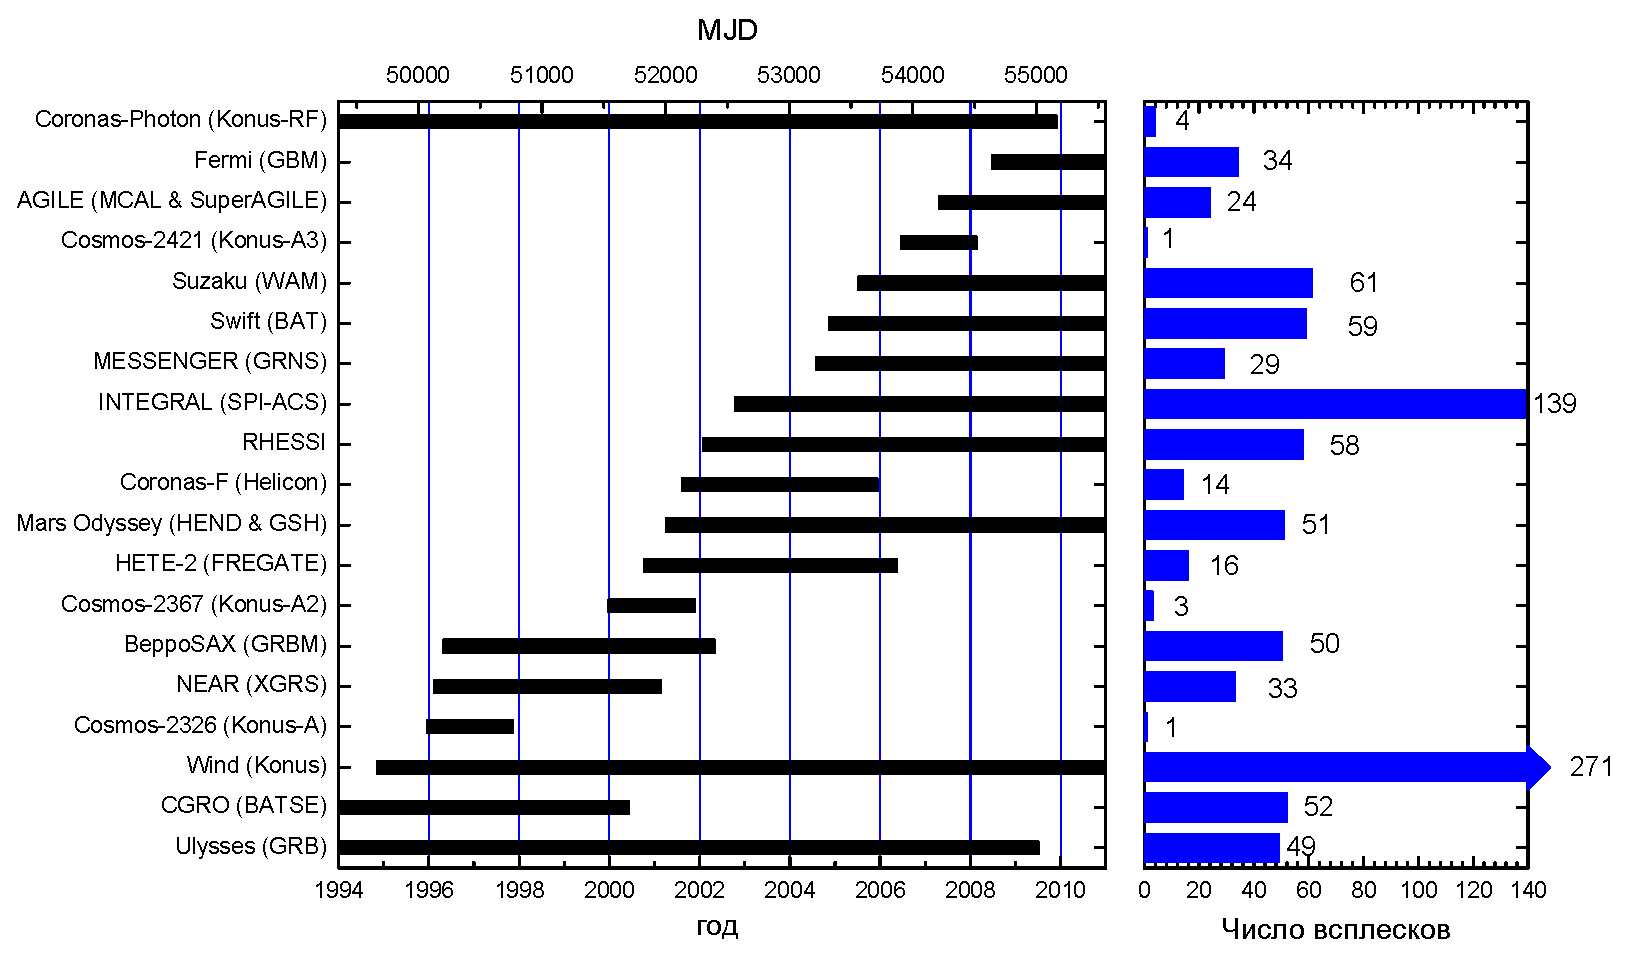
\includegraphics[width=1.0\textwidth]{Mission_timeline}}
    \caption[Время работы различных КА IPN]
  {Левая панель: сроки работы инструментов IPN с момента запуска \textit{Wind} в ноябре 1994 года 
  (имена инструментов приведены в скобках). Правая панель: число коротких всплесков KW,
  детектированных каждым инструментом (для KW~--- количество всплесков, 
  детектированных по меньшей мере одним другим КА IPN).}
  \label{img:Mission_timeline}  
\end{figure}

Данные о 271-м коротком всплеске KW представлены в таблице~3.1, размещённой 
на сайте ФТИ им. А.Ф.~Иоффе по 
ссылке~\url{http://www.ioffe.ru/LEA/shortGRBs/Catalog2/Data/tables/}.

В первой колонке приведено обозначение всплеска, <<GRBYYYYMMDD\_Tsssss>>, 
где YYYYMMDD~--- дата всплеска и sssss~--- время триггера KW в секундах UT,
округлённое до целых секунд (из-за значительного удаления \textit{Wind} от Земли
это время может отличаться на $\sim 6$~c от времени, поправленного на распространения 
сигнала от KW до центра Земли). 
Колонки (2)--(4) содержат год, месяц и число, когда произошел всплеск. 
Колонки~(5)--(7) содержат часы, минуты и секунды триггерного времени~KW.
Колонка (8) содержит Тип всплеска определенный в предыдущей главе. 
Типы имеют значения: I (результат слияния компактных объектов), 
II (результат коллапса массивной звезды), I/II (неопредёленный тип), Iee (тип I с продлённым излучением)
и Iee/II (тип не определён: Iee или~II). Колонка~(9) содержит время задержки на распространение
фронта излучения от  \textit{Wind} до центра Земли, колонки (10) и (11) содержат
$3\sigma$ ошибки этого значения (Задержки вычислены с использованием IPN локализаций приведённых ниже). 
Колонка (12) содержит названия миссий/инструментов, которые наблюдали всплеск
(также отмечены наблюдения инструментами, которые не являются часть IPN, а именно:
COMPTEL на \textit{CGRO}, DMSP, \textit{Fermi} LAT, MAXI (Monitor of All-sky X-ray Image) и SROSS)
Колонки (13)--(14) содержат полное число КА IPN и число дальних КА IPN, наблюдавших всплеск.
Последняя колонка содержит комментарий, если есть. Описание таблицы также приведено по указанной выше ссылке.

За рассматриваемый период четыре КА в межпланетном пространстве входили в состав IPN: 
\textit{Ulysses}, \textit{NEAR}, \textit{Mars Odyssey} и \textit{MESSENGER}. 
Из 271 всплеска, 30 наблюдались двумя из перечисленных КА, 102~--- одним, 
139~--- не наблюдались ни одним из указанных КА.

Семь коротких всплесков Конус-Винд были точно локализованы инструментами, 
способными строить изображения в рентгеновском или мягком гамма-диапазоне, 
а именно \textit{Swift}-BAT, \textit{HETE-2} (WXM/SXC) и \textit{INTEGRAL} (IBIS/ISGRI). 
Для большинства этих всплесков было зарегистрировано рентгеновское послесвечение; 
для некоторых из них было определено космологическое красное смещение источника 
по наблюдениям оптического послесвечения или спектроскопии родительской галактики. 
Эти всплески были использованы для проверки используемого метода триангуляции.
\FloatBarrier
\section{Методика триангуляции}
При регистрации всплеска на двух КА с временной задержкой $\delta T$, для него 
может быть построена область локализации в виде кольца на небесной сфере с углом 
раствора $\theta$ относительно вектора, соединяющего два КА. Значение угла $\theta$ определяется выражением
\begin{equation}
\cos \theta = \frac{c \delta T}{D} \mbox{ ,}
\end{equation}
где $c$~--- скорость света и $D$~--- расстояние между КА. Здесь подразумевается, 
что всплеск представляет собой плоскую волну, т.~е. расстояние до источника много больше $D$.

Измеряемая временная задержка имеет ошибку, которая в общем случае 
не симметричная $d_{\pm}(\delta T)$, т.~е. измеренная временная задержка имеет 
доверительный интервал от $\delta T + d_{-}(\delta T)$ 
до $\delta T + d_{+}(\delta T)$ ($d_{-}(\delta T)$~--- отрицательно) на заданном уровне значимости.

Полуширина кольца $d\theta_{\pm}$ определяется выражением
\begin{equation}\label{eq:CCWidth}
d\theta_{\pm} \equiv \theta_{\pm} -\theta = 
\arccos \left[ \frac{c (\delta T + d_{\mp}(\delta T))}{D} \right] - \arccos\left[ \frac{с \delta T}{D} \right]\mbox{ .}
\end{equation}

Следует отметить, что даже в случае симметричных ошибок $|d_{-}(\delta T)| = d_{+}(\delta T)$, 
кольцо может быть существенно несимметрично если $c (\delta T + d_{\pm}(\delta T))/D \sim 1$ 
(т.~е. направление на источник близк\'{о} к вектору, соединяющему два КА).

В случае $d_{\pm}(\delta T) \ll D/c$ уравнение \ref{eq:CCWidth} переходит в часто используемое выражение
\begin{equation}\label{eq:CCWidthRed}
d \theta_{\pm} = - \frac{c d_{\mp}(\delta T)}{D\sin \theta} \mbox{ .}
\end{equation}

Для вычисление наиболее вероятной временной задержки и её доверительного интервала 
был использован метод минимизации $\chi^2$, описанный в~\citep{Hurley_1999ApJSa} 
для триангуляции с дальними КА и этот же метод с некоторыми изменениями был 
использован для триангуляции с использованием KW и околоземных КА (или \textit{INTEGRAL}).

Наиболее вероятная временная задержка $\tau$ и её ошибка $d_{\pm}\tau$ между 
временными историями, записанными двумя инструментами вычислялась следующим образом. 
Пусть $n_{1,i} = n(t_{1,i})$, $n_{2,j} = n(t_{2,j})$ и 
$\sigma_{1,i}$, $\sigma_{2,j}$ обозначают числа отсчётов с вычетом фона 
и их ошибки в последовательных равномерных временных интервалах (бинах) 
$t_{1,i} = t_{1,0} + i\Delta_{1}$, $t_{2,j} = t_{2,0} + j\Delta_{2}$, 
где $i = 0,\dotsc,m_1$, $j = 0,\dotsc,m_2$; $\Delta_{1}$, 
$\Delta_{2}$~--- размеры бинов и $t_{1,0}$, $t_{2,0}$~--- времена привязки для каждого КА по всемирному времени (UT).

Для простоты будем считать, что $\Delta_1 = \Delta_2 = \Delta$ и что отсчёты детекторов 
подчиняются статистике Пуассона $\sigma_{1(2),i} = n_{\rmn{tot }1(2), i}^{1/2}$, 
где $n_{\rmn{tot }1(2), i}$~--- полное число отсчётов (источник + фон) в бине $i$. 
Предполагается, что обе временные истории содержат интересующий нас всплеск и интервалы до и после него 
(если эти интервалы отсутствуют они всегда могут быть заполнены нулями, 
а в качестве $\sigma_{1(2),i}$ взято стандартное отклонение числа отсчётов фона).
Также предполагается, что в первой временной истории $N+1$ бин, начиная 
с $i_\rmn{start}$ содержат всплеск или участок всплеска, 
который кросскоррелируется во второй временной истории. С учётом этих предположений 
можно сконструировать статистику:
\begin{equation}
R^2(\tau \equiv k\Delta) =  
\sum_{i=i_\rmn{start}}^{i=i_\rmn{start}+N} 
\frac{(n_{2,i} - s n_{1,i+k})^2}{(\sigma^2_{2,i} - s^2 \sigma_{1,i+k})} \mbox{ ,}
\end{equation}
где $s$~--- масштабный множитель являющийся отношением полного числа отсчётов, 
зарегистрированных инструментами $s = \sum_i n_{1,i} / \sum_j n_{2,j}$. 
Для идеального случая одинаковых детекторов с одинаковыми энергетическими диапазонами 
и углами падения излучения, и пуассоновской статистики отсчётов, $R^2$ распределена 
как $\chi^2$ с $N$ степенями свободы. В реальности существует несколько сложностей. 
Детекторы имеют разные энергетические диапазоны, разные аппаратные функции и работают 
в условиях с различным поведением фоновой скорости счёта (переменный фон на околоземных орбитах). 
Для коротких гамма-всплесков часть этих факторов оказывают незначительное влияние: 
вариации фона на малых временных масштабах малы, спектральная эволюция, которая 
приводит к значительному сдвигу между временными историями в различных диапазонах, 
практически отсутствует у коротких всплесков~\citep{Norris_2001grba}.

Для учёта всех отличий от идеального случая (учёта неопределённости вычисления $\tau$) 
был применён следующий метод: 
для заданного $N$ (числа бинов, используемых для построения $R^2$) вычислялось значение $\chi^2(N)$, 
соответствующие уровню значимости $3\sigma$ (соответствующие вероятности $Q(\chi^2|N)=2.7\times 10^{-3}$), 
на основе которого вычислялся соответствующий $3\sigma$ уровень значимости для приведённого $R^2_r(\equiv R^2/N)$, равный
\begin{equation}\label{eq:R3sigma}
R^2_{r,3\sigma} = \chi^2_{r,3\sigma} + R^2_{r,\rmn{min}} - 1 \mbox{ ,}
\end{equation}
где $R^2_{r,\rmn{min}}$~--- минимум $R^2_{r}(\tau)$. 
Вычитание 1 в формуле~\ref{eq:R3sigma} связано с тем, 
что $R^2_{r,\rmn{min}}\sim 1$ для идеального случая, однако, часто на практике $R^2_{r,\rmn{min}}> 1$ 
и следовательно $R^2_{r,3\sigma} > \chi^2_{r,3\sigma}$. Для определения $3\sigma$ 
доверительного интервала для $\tau$ используются ближайшие точки кривой  $R^2_{r}(\tau)$, 
лежащие выше уровня $3\sigma$ полученного из выражения~\ref{eq:R3sigma} (см. примеры на Рис.~\ref{img:CC_examples}). 
После определения кросскорреляционной задержки $\tau$ и её ошибок $d_{\pm}(\tau)$ 
может быть вычислена временная задержка $\delta T = t_{02} - t_{01} + \tau$; 
$d_{\pm}(\delta T) = d_{\pm}(\tau)$ (здесь предполагается, что абсолютные времена $t_{01}$ 
и $t_{02}$ определены точно). Далее для простоты будем называть $R^2$ как $\chi^2$.

\begin{figure}[h]
    \center{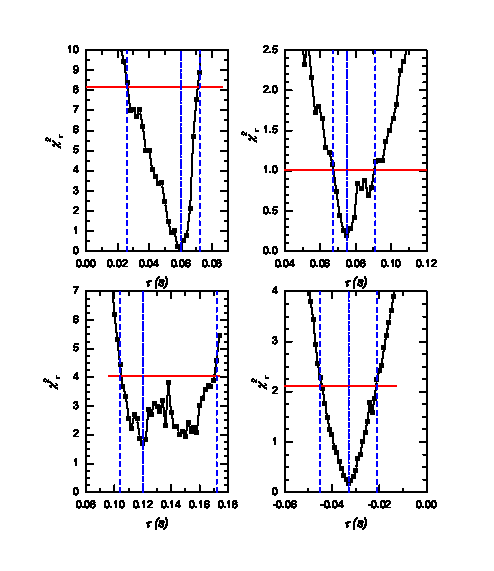
\includegraphics[width=0.75\textwidth]{gCCall}}
    \caption[Примеры кросскорреляций временных историй]
  {Примеры кросскорреляционных кривых $\chi^2_{r}(\tau)$. 
  Горизонтальные красные линии обозначают уровни $3\sigma$. 
  Вертикальные синие линии показывают наиболее вероятную кросскорреляционную задержку $\tau$ 
  (штрих-пунктирная линия) и её $3\sigma$ доверительный интервал (пунктирные линии).
  Вверху слева: GRB19971118\_T29008. Кросскорреляция временной истории KW (2~мс) с временной историей BATSE (64~мс),
  $\tau = 0.060 (-0.034,+0.012)$~с ($\rmn{dof} = 2$). 
  Вверху справа: GRB20070321\_T67937. Кросскорреляция временной истории KW (2~мс) с временной историей WAM (1/64~с),
  $\tau = 0.075 (-0.008,+0.016)$~с ($\rmn{dof} = 12$). 
  Внизу слева: GRB20090715\_T62736. Кросскорреляция временной истории KW (2~мс) с временной историей SPI-ACS (50~мс),
  $\tau = 0.120 (-0.016,+0,052)$~с ($\rmn{dof} = 7$). 
  Внизу справа: GRB20100206\_T48606. Кросскорреляция временной истории GBM (1~мс)с временной историей KW (2~мс),
  $\tau = -0.033 \pm 0.012$~с ($\rmn{dof} = 9$).
  }
  \label{img:CC_examples}  
\end{figure}
\FloatBarrier

\section{Триангуляционные кольца}
Используя приведённую выше методику для 271-го короткого всплеска Конус-Винд было 
получено одно или более триангуляционное кольцо. Обсуждение деталей получения 
временных задержек для различных пар КА приведены в нижеследующих разделах.

\subsection{Кольца, полученные с использованием дальних КА}
Дальние КА (КА в межпланетном пространстве) играют важную роль в триангуляции 
гамма-всплесков. Их длинная база позволяет получать малые области локализации 
для большого числа всплесков. Однако детекторы на этих КА обычно меньше, чем на 
околоземных, при этом часть детекторов предназначены для планетарных исследований 
с возможностью регистрации гамма-всплесков. Эти детекторы могут иметь более 
грубое временное разрешение и меньшую чувствительность. Также часы на этих КА 
не всегда калиброваны по Всемирному координированному времени (UTC) настолько точно, 
насколько часы на околоземных КА (или их калибровка не может быть определена настолько аккуратно).

Для локализации использовались данные четырёх межпланетных КА: \textit{Ulysses}, 
\textit{NEAR}, \textit{Mars Odyssey} и \textit{MESSENGER}. Из них только \textit{Ulysses} 
имел эксперимент, посвященный гамма-всплескам. Временное разрешение этих четырёх 
экспериментов составляло от 32~мс (триггерный режим \textit{Ulysses}) 
до 1~с (\textit{MESSENGER}, \textit{NEAR}). При регистрации короткого всплеска 
детектором с разрешением, намного превышающим длительность всплеска, обычно 
наблюдается превышение скорости счёта в одном бине, при этом неопределённость 
временной задержки составляет половину от наибольшего временного разрешения. 
Точность часов КА определялась двумя способами. 
В случае \textit{Ulysses}, эксперименту, регистрирующему гамма-всплески, 
в точно известные моменты времени посылались определённые команды. 
Учитывая аберрационное время и задержки выполнения команд на борту КА, 
можно было уточнить временную привязку с точностью от нескольких миллисекунд 
до 125~мс. 
%(хотя точность привязки предполагалась равной нескольким миллисекундам, 
%зачастую технические сложности не давали возможность её проверить). 
Дополнительно точность временной привязки межпланетных КА может быть проверена 
триангуляцией известных источников, чьё положение хорошо известно из других измерений: 
это могут быть как источники мягких повторяющихся гамма-всплесков 
(другие употребляемые названия этих объектов: мягкие гамма-репитеры; SGRs), 
так и гамма-всплески локализованные \textit{Swift}-XRT 
или \textit{Swift}-UVOT. При вычислении кросскорреляционной задержки коротких всплесков
использовалась консервативная оценка ошибок, считалось, 
что ошибка $\tau$ на уровне $3\sigma$ не может быть меньше 125~мс.

Всего 132 коротких всплеска KW наблюдались дальними КА: 30 наблюдались 
двумя дальними КА и 102 одним дальним КА. Среди них девять были точно локализованы 
инструментами, способными строить изображения в рентгеновском или мягком гамма-диапазоне. 
Без учёта этих всплесков было получено 150 колец. Распределение $3\sigma$ полуширин 150 колец 
представлено на Рис.~\ref{img:dist_150}. Наименьшая полуширина $0\fdg0024$ (0\farcm14), 
наибольшая $2\fdg21$, средняя $0\fdg099$ ($5\farcm9$), геометрическое 
среднее $0\fdg028$ ($1\farcm7$).

\begin{figure}[h]
    \center{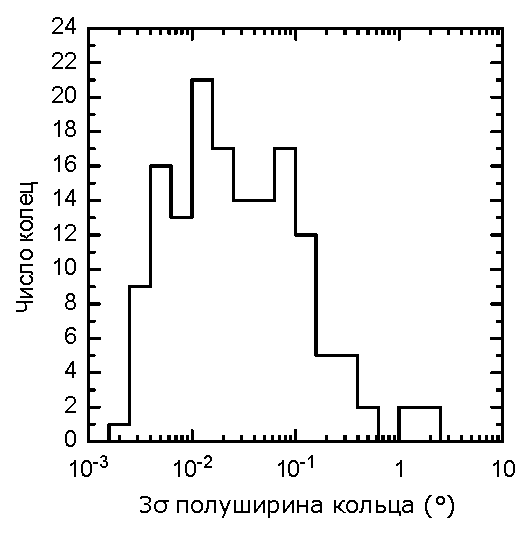
\includegraphics[width=0.5\textwidth]{dN_150_annuli_distant}}
    \caption[Распределение ширин колец, построенных с использованием дальних КА]
    {Распределение $3\sigma$ полуширин 150 триангуляционных колец, полученных с 
    использованием данных дальних КА.}
 \label{img:dist_150}  
\end{figure}
\FloatBarrier
\subsection{Кольца, полученные с использованием KW, \textit{INTEGRAL} и околоземных КА}
KW занимает особое место в IPN благодаря уникальному набору характеристик: 
непрерывному обзору всего неба двумя спектрометрами, положению в межпланетном 
пространстве в условиях исключительно стабильного фона, широкому энергетическому 
диапазону (10~кэВ--10~МэВ номинальный; $\sim 20$~кэВ--15~МэВ в 2010~г.) и достаточно 
высокой чувствительности ($\sim 10^{-7}$~эрг~см$^{-2}$). Доля времени наблюдения 
KW, отнесённая ко всему времени работы, составляет примерно 95\%. 
Эксперимент зарегистрировал большую часть событий IPN, являясь важным компонентом 
IPN на расстоянии $\simeq 1\textrm{--}7$ световых секунды (см. Рис.~\ref{img:Wind_distance}).

\begin{figure}[h]
    \center{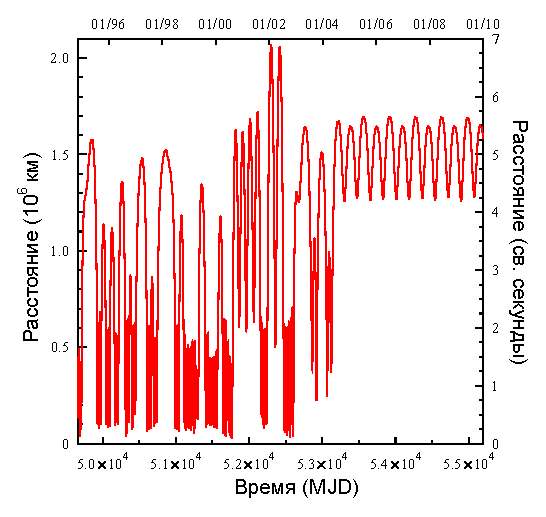
\includegraphics[width=0.5\textwidth]{Wind_distance}}
    \caption[Расстояние \textit{Wind} от Земли]
    {Зависимость расстояния \textit{Wind} от Земли от времени.
     Максимальное расстояние составляло 7 световых секунд с января по май 2002 г., 
     когда КА находился на далекой орбите (distant prograde orbit, DPO).
     С 2004~г. \textit{Wind} находится на орбите Лиссажу вокруг точки либрации $L_1$
     в системе Солнце-Земля на расстоянии 5 световых секунд.}
 \label{img:Wind_distance}  
\end{figure}

В триггерном режиме временное разрешение KW составляет 2~мс на интервале 
от $T_0-0.512$~с до $T_0+0.512$~с ($T_0$~--- время срабатывания триггера), 
который покрывает, в большинстве случаев, весь короткий всплеск или, по крайней 
мере, его наиболее интенсивную часть, позволяя производить точную кросс-корреляцию 
с временными историями других инструментов. Погрешность часов KW составляет 
менее 1~мс и их точность была проверена триангуляцией всплесков от SGRs 
и точно локализованных гамма-всплесков.

Наибольшую точность кросс-корреляции с KW (наименьшие неопределённости 
времени задержки) дают околоземные КА с большими эффективными площадями, 
а именно: \textit{CGRO}~(BATSE), \textit{BeppoSAX}~(GRBM), \textit{INTEGRAL}~(SPI-ACS), 
\textit{Suzaku}~(WAM), \textit{Swift}~(BAT), и \textit{Fermi}~(GBM). 
В настоящее время кросс-корреляции с \textit{Fermi}~(GBM) обычно даёт наилучший 
результат (наиболее узкое кольцо) благодаря схожим детекторам (сцинтилляционные 
спектрометры на основе NaI(Tl)), большой эффективной площади GBM 
(несколько сотен см$^2$ при использовании нескольких детекторов) и временной 
привязке каждого фотона в 128 энергетических каналах, что позволяет получать 
временную историю GBM с любым временным разрешением и в том же спектральном диапазоне, 
что у KW.

Так как часы на большинстве околоземных КА очень точные, высокая статистика 
отсчётов в сумме с высоким временным разрешением дают ошибки временных задержек 
вплоть до нескольких миллисекунд. Таким образом, несмотря на достаточно небольшое 
расстояние между околоземными КА и KW в несколько световых секунд, 
получаемая относительная ошибка временной задержки ($c d_{\pm}(\delta T)/D$), 
которая определяет ширину кольца (см. Уравнения~\ref{eq:CCWidth} и~\ref{eq:CCWidthRed}) 
может быть сравнима или даже меньше, чем для кольца с дальним КА. Подобные малые ошибки, 
порядка нескольких миллисекунд, и следовательно узкие кольца, могут быть получены 
для коротких всплесков с острым пиком или быстрым нарастанием/спадом. 
С другой стороны, всплески с плавными импульсами дают достаточно большие ошибки 
времени задержки, и следовательно более широкие кольца.

Для KA \textit{Wind}, \textit{INTEGRAL} и околоземных аппаратов, неопределённости эфемерид 
незначительны по сравнению с ошибками времён задержки и поэтому они не учитываются 
при построении триангуляционных колец.

Всего было получено 356 колец для Конус-Винд и околоземных КА, и Конус-Винд и 
\textit{INTEGRAL}. На Рис.~\ref{img:dist_356} представлено распределение ошибок временных 
задержек и $3\sigma$ полуширин этих колец. Наименьшая неопределённость времени 
задержки составляет 2~мс, наибольшая -- 504~мс, средняя -- 43~мс и средняя 
геометрическая~--- 23~мс. Наименьшая $3\sigma$ полуширина кольца составляет 
$0\fdg027$~($1\farcm6$), наибольшая~--- $32\fdg2$, 
средняя~--- $1\fdg3$ и средняя геометрическая~--- $0\fdg43$.

В последующих подразделах приведены некоторые детали триангуляции с использованием 
KW и \textit{INTEGRAL} и околоземных КА.

\begin{figure}[h]
    \center{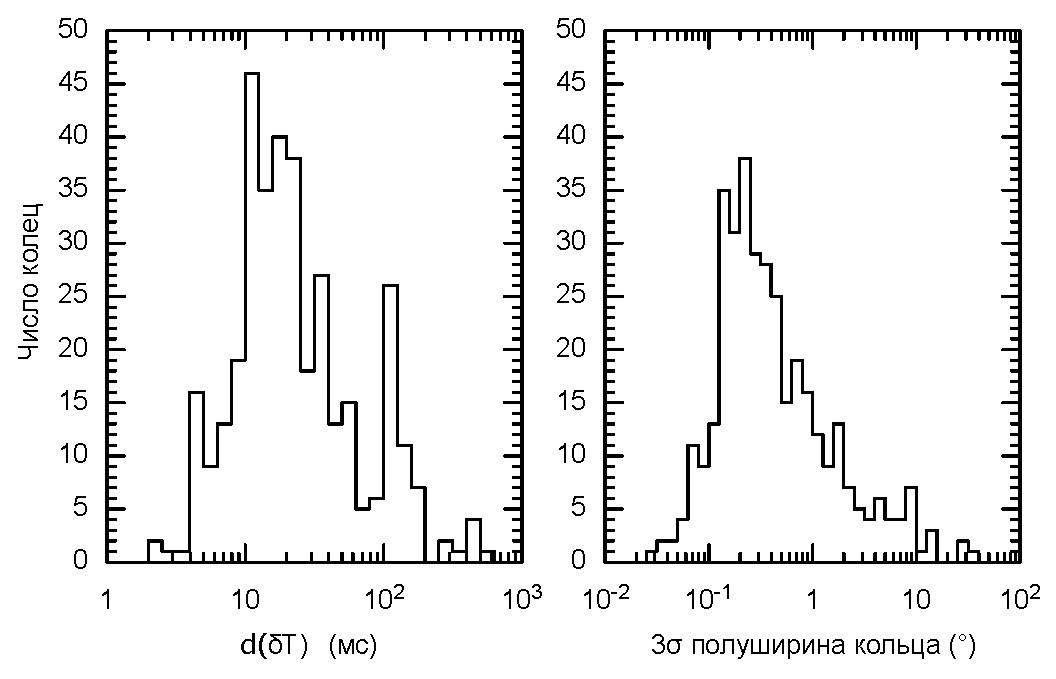
\includegraphics[width=0.75\textwidth]{dN_356_annuli}}
    \caption[Распределение ширин колец, построенных с использованием околоземных КА]
    {Распределение неопределенности времени задержки $d(\delta T) \equiv (\delta T_{+} + |\delta T_{-}|)/2$
    и $3\sigma$ полуширины для 356 триангуляционных колец, полученных с использованием данных
    KW и околоземного КА (или INTEGRAL).}
 \label{img:dist_356}  
\end{figure}
\FloatBarrier
\subsubsection{Триангуляции KW--\textit{CGRO}~(BATSE)}\label{sec:KW_BATSE_cc}
Эксперимент BATSE был установлен на обсерватории имени Комптона и предназначен 
для исследований в области астрофизики высоких энергий~\citep{Fishman_1992NASCP3137}. 
Его детекторы большой площади (Large Area Detectors) записывали временные истории 
гамма-всплесков в четырёх энергетических диапазонах: Ch1, Ch2, Ch3, Ch4 с номинальными 
границами каналов: 25--55~кэВ, 55--110~кэВ, 110--320~кэВ и $>320$~кэВ. 
Часы на борту \textit{CGRO} имели точность 100~мкс, которая проверялась при помощи 
тайминга пульсаров. Бортовое программное обеспечение увеличивало эту ошибку, 
давая неопределённость в триггерных временах BATSE до $\simeq 1$~мс.

BATSE зарегистрировал 52 коротких всплеска Конус-Винд: 44 в триггерном режиме 
и 8 в режиме реального времени (real-time mode), в котором ведётся непрерывная 
запись скорости счёта с разрешением 0.25, 0.5, 1 или 2~с в зависимости от скорости 
передачи информации. Триангуляционные кольца были получены для 44 всплесков, 
зарегистрированных в триггерном режиме, и 6 всплесков, зарегистрированных в 
режиме реального времени (эти всплески наблюдались только Конус-Винд и BATSE).

Для кросс-корреляции с триггерными всплесками BATSE использовались временные 
истории KW в диапазонах G2+G3 или G2 с временным разрешением 2 или 16~мс 
и объединённые временные истории BATSE (объединение типов данных DISCLA, PREB 
и DISCS~\citep{Fishman_1992NASCP3137}) в диапазонах Ch2+Ch3+Ch4 или Ch2+Ch3 
с временным разрешением 64~мс. Для нескольких всплесков такие временные истории 
были недоступны и были использованы другие типы данных BATSE. Обычно делались 
кросс-корреляции для различных комбинаций каналов для проверки согласия 
получаемых временных задержек и выбиралась та, для которой $\chi^2$ был наименьший. 
Кросскорреляционные кривые для различных диапазонов могут быть сдвинуты относите
льно друг друга (на несколько миллисекунд), но $3\sigma$ интервалы для 
кросскорреляционной задержки $\tau$ всегда согласуются хорошо.

Полученные $\chi^2_{r,\rmn{min}}$ находятся в диапазоне от 0.06 до 4.51 со 
средним 0.81. Максимальное $\chi^2_{r,\rmn{min}}=4.51$~(dof=6)~--- явный выброс 
в распределении всплесков по $\chi^2_{r,\rmn{min}}$.

Это значение соответствует особенно сильному всплеску GRB19970704\_T04097 
(триггер BATSE \#6293) с пиковой скоростью счёта $1.8\times10^5$~отсчётов~с$^{-1}$ 
на масштабе 2~мс на KW и $6.9\times10^5$~отсчётов~с$^{-1}$ на масштабе 64~мс у BATSE. 
Обе временные истории существенно искажены эффектами мёртвого времени и наложения 
импульсов (когда два фотона считаются как один с суммарной энергией). 
Полученная статистическая ошибка задержки для этого всплеска составила всего 3~мс, 
для учёта описанных эффектов была добавлена систематическая ошибка 6~мс.

Полученные ошибки временных задержек находятся в диапазоне от 5~мс до 84~мс со 
средним 24~мс и геометрическим средним 18~мс. Полученные $3\sigma$ полуширины  
колец находится в диапазоне от $0\fdg082$ до $11\fdg0$ 
со средним $1\fdg14$ и геометрическим средним $0\fdg60$. 
Наиболее широкое кольцо с $3\sigma$ полушириной $11\fdg0$ получено 
для GRB19991001\_T04950 (триггер BATSE \#7781), в это время \textit{Wind} находился 
всего в 0.34~световых секунды от Земли.

Расстояния между центральными линиями колец KW--BATSE и центрами локализаций 
BATSE находятся в диапазоне от $0\fdg007$ до $7\fdg7$ 
со средним $2\fdg23$ и геометрическим средним $0\fdg60$. 
Для 14 всплесков $1\sigma$ круговая область локализации BATSE не пересекает кольца 
KW--BATSE и расстояния от ближайшей границы кольца находятся в диапазоне 
от $1.02\sigma$ до $7.2\sigma$. Из 52 всплесков 16 наблюдались только Конус-Винд 
и BATSE и 12 наблюдались только Конус-Винд, BATSE и \textit{BeppoSAX}. Для этих 
всплесков область локализации была получена в виде сегмента кольца KW--BATSE 
с использованием следующего метода. В качестве центра сегмента выбиралась точка 
на центральной линии кольца ближайшая к центру локализации BATSE, и в качестве 
углов сегмента выбирались точки пересечения кольца и окружности с центром в этой 
точке и с радиусом равным сумме удвоенной $1\sigma$ ошибки локализации BATSE, 
систематической ошибки, взятой равной $2\fdg0$ и расстояния между 
центром локализации BATSE и центральной линией кольца. Иллюстрация метода приведена 
на Рис.~\ref{img:IPN_BATSE_loc}. Систематическая ошибка локализаций BATSE $\simeq 2^{\circ}$ 
была обнаружена в работе~\citep{Briggs_1999ApJS}.

\begin{figure}[h]
    \center{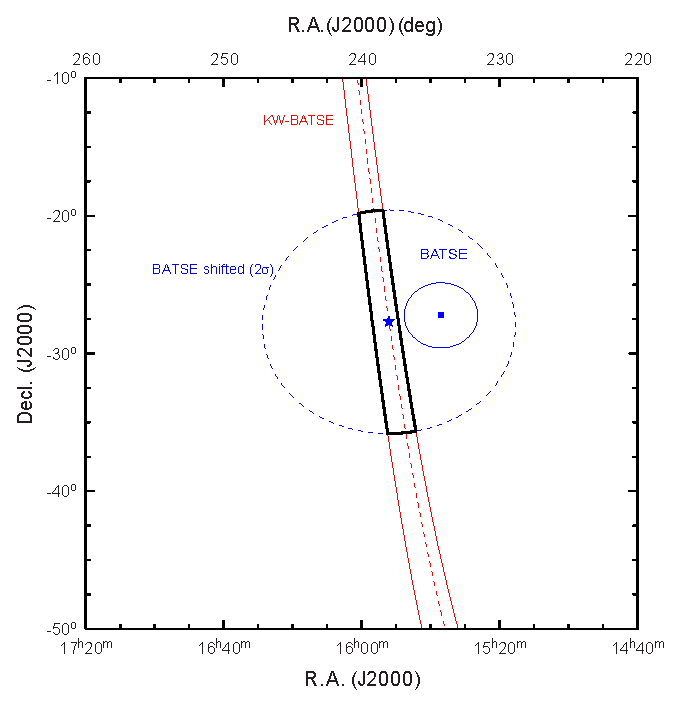
\includegraphics[width=0.5\textwidth]{IPN_BATSE_loc}}
    \caption[IPN/BATSE локализация GRB19960420\_T16844 (BATSE \#5439)]
    {IPN/BATSE локализация GRB19960420\_T16844 (BATSE \#5439). 
    Центр локализации BATSE 
    (R.A., decl.(J2000), Err = $ 234\fdg25$, $-27\fdg23$, $2\fdg37$)
    лежит в $3\fdg38$ от центральной линии кольца KW-BATSE.
    Полученный протяженный бокс показан сплошной черной линией и его центр 
    (то есть, ближайшая к центру локализации BATSE точка на центральной линии кольца) обозначена звездочкой. 
    Углы бокса образованы пересечением окружности с центром, отмеченным звездочкой, и
    радиусом $8\fdg12$, то есть суммой $2\sigma$ радиуса локализации BATSE
    и $3\fdg38$ систематической ошибки (пунктирная линия), и кольца KW-BATSE.
    }
 \label{img:IPN_BATSE_loc}  
\end{figure}
\FloatBarrier
\subsubsection{Триангуляции KW--\textit{Fermi}~(GBM)}
Инструмент GBM на борту обсерватории \textit{Fermi} предназначен для изучения 
гамма-всплесков в диапазоне $\sim8$~кэВ--40~МэВ~\citep{Meegan_2009ApJ}. 
Преимущества GBM состоят в высокой эффективной площади и возможности временной 
привязки каждого фотона (Time-tagged events, TTE данные). Часы на борту GBM имеют 
точность временной привязки превышающую 20~мкс. TTE данные содержат отсчёты в 128 
энергетических каналах от $\sim5$~кэВ--2~МэВ, что даёт возможность получить 
временную историю в тех же энергетических диапазонах что и на Конус-Винд.

Инструмент GBM наблюдал 34 коротких всплеска Конус-Винд, для всех из них были 
получены триангуляционные кольца. Для кросс-корреляции с триггерными всплесками 
BATSE использовались временные истории Конус-Винд в диапазонах G2+G3 или G2 с 
временным разрешением 2 или 16~мс и временные истории GBM с разрешением от 1 до 
16~мс созданные из TTE данных только NaI детекторов.

Полученные $\chi^2_{r,\textrm{min}}$ находятся в диапазоне от 0.16 до 2.10 со средним 0.9. 
Полученные ошибки времён задержки лежат в диапазоне 2.5~мс до 136~мс со средним 22~мс и 
геометрическим средним 15~мс. Полученные $3\sigma$ полуширины  колец находится в 
диапазоне от $0\fdg035$~($2\farcm1$) до $1\fdg65$ 
со средним $0\fdg35$ и геометрическим средним $0\fdg23$.

\subsubsection{Триангуляции KW--\textit{INTEGRAL}~(SPI-ACS)}
Помимо своего прямого назначения~--- отсечения фоновых событий германиевого 
спектрометра инструмента SPI, защита ACS используется как в качестве всенаправленного 
детектора гамма-всплесков~\citep{von_Kienlin_2003AA}. Инструмент измеряет временные 
истории гамма-всплесков с временным разрешением 50~мс в одном энергетическом 
диапазоне выше $\sim 80$~кэВ (подробнее см. в~\citep{Lichti_2000AIPC}). 
Систематическая ошибка $125\pm10$~мкс во временной привязке ACS была обнаружена~\citep{Rau_2004GCN} 
и начиная с апреля 2004~г. все временные истории SPI-ACS корректируются автоматически; 
корректировка для предшествующих данных была выполнена вручную.

Систематическая ошибка связана с тем что преобразование из бортового времени в UTC 
происходило приближенно при получении временных историй SPI-ACS в реальном времени 
(в пределах нескольких секунд после триггера \url{ftp://isdcarc.unige.ch/arc/FTP/ibas/spiacs/}). 
С другой стороны, преобразование времени, использовавшиеся для архивных и данных и данных, 
приходящих с задержкой, является точным. Также было показано, что дрейф часов ACS 
по отношению к часам германиевого детектора составляет в течении всей миссии 
составило $\sim 1$~мс~\citep{Zhang_2010int}, таким образом уменьшив систематическую 
ошибку временной привязки ACS с 10~мс до 1~мс.

Временные истории SPI-ACS, скорректированные на систематические сдвиги и имеющие 
высокую точность привязки (по крайней мере с точность вплоть до 1~мс), доступны 
в архиве данных \textit{INTEGRAL} начиная с версии 3. Архивные и данные, приходящие 
с задержкой, с одинаковой точностью временной привязки (приходящие в пределах 
часа после регистрации всплеска) доступны на ресурсе 
\url{http://isdc.unige.ch/~savchenk/spiacs-online/} и 
\url{http://www.isdc.unige.ch/heavens/}. 
Эти данные систематически используются для оперативной триангуляции.

Инструмент SPI-ACS зарегистрировал 139 коротких всплеска Конус-Винд, из них 
для 103 были получены триангуляционные кольца. Для кросс-корреляции использовались 
временные истории Конус-Винд в диапазонах G2+G3 или G3 с временным разрешением 2 или 16~мс.

Полученные $\chi^2_{r,\textrm{min}}$ находятся в диапазоне от 0.04 до 3.96 со средним 1.02. 
Полученные ошибки задержек лежат в диапазоне 4~мс до 175~мс со средним 24~мс 
и геометрическим средним 19~мс. Полученные $3\sigma$ полуширины колец находится 
в диапазоне от $0\fdg047$~($2\farcm8$) до $4\fdg3$ 
со средним $0\fdg41$ и геометрическим средним $0\fdg29$.

\subsubsection{Триангуляции KW--\textit{Suzaku}~(WAM)}
Инструмент WAM является активной защитой детектора жесткого рентгеновского 
излучения на борту миссии \textit{Suzaku}~\citep{Yamaoka_2009PASJ}. В триггерном 
режиме WAM записывает временные истории всплесков с временным разрешением 1/64~с 
в четырёх каналах в диапазоне $\approx50$--5000~кэВ. В режиме реального времени 
разрешение составляет 1~с. В работе~\citep{Yamaoka_2009PASJ} было показано, 
что систематическая ошибка временной привязки \textit{Suzaku}~(WAM) пренебрежимо мала.

Инструмент WAM зарегистрировал 61 короткий всплеск Конус-Винд: 51 в триггерном 
режиме и 10 в режиме реального времени. Кольца были получены для 45 триггерных всплесков.

Для кросс-корреляции использовались временные истории Конус-Винд в 
диапазонах G2+G3 или G3 с временным разрешением 2 или 16~мс и временные истории 
WAM в сумме четырёх диапазонов детектора с наиболее сильным откликом.

Полученные $\chi^2_{r,\textrm{min}}$ находятся в диапазоне от 0.21 до 1.78 со средним 1.03. 
Полученные ошибки задержек лежат в диапазоне от 4~мс до 104~мс со средним 20~мс 
и геометрическим средним 14~мс. Полученные $3\sigma$ полуширины колец находятся 
в диапазоне от $0\fdg060$~($3\farcm6$) до $2\fdg44$ 
со средним $0\fdg30$ и геометрическим средним $0\fdg21$.

\subsubsection{Триангуляции KW--\textit{BeppoSAX}~(GRBM)}
Инструмент \textit{BeppoSAX}~(GRBM) являлся защитой, работающей по принципу 
антисовпадения, системы детектирования гамма квантов PHOSWICH 
(PHOSphor sandWICH)~\citep{Feroci_1997SPIE, Frontera_1997AAS}. В триггерном режиме 
инструмент измерял временные истории с разрешением 7.8125~мс в диапазоне 40--700~кэВ; 
в режиме реального времени разрешение составляло 1~с.

Инструмент GRBM зарегистрировал 50 коротких всплесков Конус-Винд: 41 в триггерном 
режиме и 9 в режиме реального времени. Триангуляционные кольца были получены для 38 всплесков,
зарегистрированных в триггерном режиме и для одного всплеска, зарегистрированного 
в режиме реального времени (этот всплеск наблюдался только Конус-Винд и GRBM).

Для кросс-корреляции использовались временные истории Конус-Винд в диапазонах G2 
или G2+G3 с временным разрешением 2 или 16~мс и временные истории GRBM, 
приведённые к разрешению 32~мс.

Полученные $\chi^2_{r,\textrm{min}}$ находятся в диапазоне от 0.25 до 12.1 со 
средним 1.43. Максимальный $\chi^2_{r,\textrm{min}}$ равный 12.1 (dof=6) 
соответствует исключительно интенсивному событию GRB19970704\_T04097 с пиковой 
скоростью счёта $1.8\times10^5$~отсчётов~с$^{-1}$ на Конус-Винд на масштабе 2~мс 
и $1.5\times10^5$~отсчётов~с$^{-1}$ в GRBM на масштабе 32~мс. Обе временные истории 
существенно искажены эффектами мёртвого времени и наложения импульсов 
(когда два фотона считаются как один с суммарной энергией). Полученная статистическая 
ошибка задержки для этого всплеска составила всего 2~мс, для учёта описанных 
эффектов ошибка была увеличена до 6~мс.

Полученные ошибки задержек лежат в диапазоне от 4.5~мс до 216~мс со средним 32~мс 
и геометрическим средним 18~мс.

Сравнение первоначально полученных колец с другими кольцами IPN, так же как 
сравнение временных историй GRBM и BATSE выявило систематический сдвиг во 
временной привязке GRBM доходящий до 100~мс. Так как этот сдвиг варьируется от 
всплеска к всплеску, для триангуляции KW--GRBM была введена 100~мс 
систематическая ошибка. Это привело к существенному уширению колец. Таким образом, 
конечные $3\sigma$ полуширины колец находятся в диапазоне от $1\fdg23$ 
до $32\fdg2$ со средним $5\fdg30$ и геометрическим 
средним $3\fdg87$.

\subsubsection{Триангуляции KW--\textit{Swift}~(BAT)}
\textit{Swift}~(BAT) -- высокочувствительный телескоп с кодирующей маской с 
широким полем зрения, который регистрирует гамма-всплески в реальном 
времени~\citep{Barthelmy_2005SSRv}. Если всплеск происходит вне поля зрения, 
он не может быть локализован, но временная история BAT может быть использована 
для триангуляции. Для таких всплесков всегда доступна временная история 
с разрешением 64~мс в четырёх стандартных диапазонах BAT (15--25~кэВ, 25--50~кэВ, 
50--100~кэВ и 100-350~кэВ). Для некоторых всплесков доступны TTE данные, что 
даёт возможность получить временную историю с любым необходимым разрешением.

Инструмент BAT зарегистрировал 44 коротких всплеска Конус-Винд вне поля зрения, 
для 23 из них были получены триангуляционные кольца.

Для кросс-корреляции использовались временные истории Конус-Винд в диапазонах G2 
или G2+G3 с временным разрешением 2 или 16~мс и временные истории BAT с разрешением 
64~мс в большинстве случаев в диапазоне выше 50~кэВ, что обычно даёт лучшее 
отношение сигнал-шум и лучшее соответствует диапазону Конус-Винд.

Полученные $\chi^2_{r,\textrm{min}}$ находятся в диапазоне от 0.25 до 7.48 со 
средним 1.41. Максимальный $\chi^2_{r,\textrm{min}}$ равный 12.1 (dof=6) 
соответствует исключительно интенсивному всплеску GRB20060306\_T55358 с сильной 
спектральной эволюцией и пиковой скоростью счёта $1.9\times10^5$~отсчётов/с 
на Конус-Винд на масштабе 2~мс. Полученная статистическая ошибка задержки 
для этого всплеска составила всего 5~мс, для учёта описанных эффектов была 
добавлена систематическая ошибка 10~мс.

Полученные ошибки временных задержек лежат в диапазоне от 5~мс до 64~мс со 
средним 22~мс и геометрическим средним 18~мс. Полученные $3\sigma$ полуширины 
колец находятся в диапазоне от $0\fdg059$~($3\farcm5$) 
до $1\fdg18$ со средним $0\fdg41$ 
и геометрическим средним $0\fdg29$.

\subsubsection{Триангуляции KW--\textit{Коронас-Ф} (Геликон)}
Гамма спектрометр Геликон, установленный на солнечной обсерватории Коронас-Ф, 
имел схожие с  Конус-Винд характеристики детекторов и типы научных данных. 
Схожее устройство двух инструментов позволило получить хорошие кросс-корреляции 
временных историй всплесков.

Геликон зарегистрировал 14 коротких всплесков Конус-Винд, для всех из них были 
получены кольца KW--Геликон.

Полученные $\chi^2_{r,\textrm{min}}$ находятся в диапазоне от 0.25 до 2.67 со средним 1.02. 
Полученные ошибки временных задержек лежат в диапазоне от 4~мс до 80~мс со средним 25~мс 
и геометрическим средним 17~мс. Полученные $3\sigma$ полуширины колец находятся 
в диапазоне от $0\fdg045$~($2\farcm7$) до $1\fdg15$
со средним $0\fdg38$ и геометрическим средним $0\fdg25$.

\subsubsection{Триангуляции KW--\textit{Космос}~(Конус-А, А2, А3)}
Гамма спектрометры Конус-А, Конус-А2 и Конус-А3 были установлены на КА 
\textit{Космос} -2326, -2367 и -2421. Краткое описание инструмента Конус-А дано в~\citep{Aptekar_1998ApJ}, 
инструменты Конус-А2 и Конус-А3 имели схожее устройство и типы научных данных.

Этими инструментами было зарегистрировано в триггерном режиме пять коротких 
всплесков Конус-Винд. Триангуляционные кольца KW--\textit{Космос} были 
получены для четырёх из них.

Полученные $\chi^2_{r,\textrm{min}}$ находятся в диапазоне от 0.73 до 1.42 со средним 1.07. 
Полученные ошибки временных задержек лежат в диапазоне от 4~мс до 56~мс со средним 35~мс. 
Полученные $3\sigma$ полуширины колец находятся в диапазоне от $0\fdg15$ 
до $1\fdg20$ со средним $0\fdg79$.

\subsubsection{Триангуляции KW--\textit{RHESSI}}
Гамма спектрометр высокого разрешения \textit{RHESSI} предназначен для изучения 
излучения высоких энергий от солнечных вспышек в широком диапазоне энергий 
от 3~кэВ до 17~МэВ~\citep{Lin_2002SoPh, Smith_2002SoPh}. Данные накопленные в режиме TTE 
позволяют получить произвольную временную и спектральную группировку зарегистрированных квантов.

Инструмент \textit{RHESSI} зарегистрировал 58 коротких всплесков Конус-Винд, из 
них для 32 были получены кольца KW--\textit{RHESSI}.

Для кросс-корреляции использовались временные истории Конус-Винд 
в диапазонах G2, G1+G2 или G2+G3 с временным разрешением 2, 16, 64 или 256~мс, 
в зависимости от интенсивности всплеска.

Полученные $\chi^2_{r,\textrm{min}}$ находятся в диапазоне от 0.36 до 2.62 со 
средним 1.07. Полученные ошибки временных задержек лежат в диапазоне от 2~мс 
до 184~мс со средним 36~мс и геометрическим средним 20~мс. Полученные $3\sigma$ 
полуширины колец находятся в диапазоне от $0\fdg027$~($1\farcm6$) 
до $2\fdg71$ со средним $0\fdg53$ 
и геометрическим средним $0\fdg30$.

\subsubsection{Триангуляции KW--\textit{HETE-2} (FREGATE)}
Гамма спектрометр FREGATE на борту \textit{HETE-2} был предназначен для регистрации 
гамма-всплесков в диапазоне энергий 8--400~кэВ~\citep{Ricker_2003AIPC, Atteia_2003AIPC}. 
В триггерном режиме он записывал временные истории гамма-всплесков с временным 
разрешением 1/32~с в диапазоне 8--400~кэВ, помимо этого велась непрерывная запись 
скорости счёта с разрешением 0.1638~с.

Инструмент FREGATE зарегистрировал 16 коротких всплесков KW: 8 в триггерном режиме 
и 8 в режиме непрерывной записи. В большинстве случаев отклик FREGATE был существенно
слабее чем у других инструментов, установленных на КА с низкими околоземными орбитами, 
поэтому данные FREGATE использовались нескольких случаях, года ни один другой КА на низкой 
орбите не детектировал данный всплеск. Кольца KW--FREGATE были получены для четырёх 
всплесков, зарегистрированных в триггерном режиме.

Для кросс-корреляции использовались временные истории KW в диапазонах G2 
или G2+G3 с временным разрешением 2 или 16~мс.

Полученные $\chi^2_{r,\textrm{min}}$ находятся в диапазоне от 0.50 до 1.43 со средним 0.96. 
Полученные ошибки временных задержек лежат в диапазоне от 56~мс до 168~мс со средним 102~мс. 
Полученные $3\sigma$ полуширины колец находятся в диапазоне от $0\fdg95$ 
до $1\fdg47$ со средним $1\fdg10$.

\subsubsection{Триангуляции KW--\textit{AGILE}~(MCAL)}
Гамма спектрометр MCAL на борту миссии \textit{AGILE} чувствителен к гамма-квантам 
с энергией $\approx 0.35$--100~МэВ~\citep{Tavani_2009AA}. Запись временных историй 
гамма-всплесков в триггерном режиме ведётся в формате TTE.

Инструмент MCAL зарегистрировал 24 коротких всплесков KW: 22 в триггерном 
режиме и 2 в режиме непрерывной записи. Во многих случаях отклик MCAL оказывался 
слабым из-за его высокого энергетического порога и сильного экранирования инструментом GRID, 
поэтому MCAL использовался для триангуляции сильных всплесков. В сумме было получено девять колец
KW--MCAL.

Для кросс-корреляции использовались временные истории KW в диапазонах G3 
или G2+G3 с временным разрешением 2 или 16~мс.

Полученные $\chi^2_{r,\textrm{min}}$ находятся в диапазоне от 0.29 до 2.26 со 
средним 1.08. Полученные ошибки временных задержек лежат в диапазоне от 5~мс 
до 21~мс со средним 13~мс. Полученные $3\sigma$ полуширины колец находятся 
в диапазоне от $0\fdg071$~($4\farcm3$) до $0\fdg06$ 
со средним $0\fdg21$.

\subsubsection{Триангуляции \textit{INTEGRAL}--околоземные КА}
Даже без планетарных миссий, мини-сеть КА на низких околоземных орбитах, 
плюс \textit{INTEGRAL} и KW, часто позволяют получить область локализовать 
гамма-всплеска. Так как орбита \textit{INTEGRAL} расположена на расстояниях 
$\lesssim 0.5$~световых секунд, что гораздо меньше расстояния Земля--\textit{Wind} 
$\simeq 5$~световых секунд, кольца KW--\textit{INTEGRAL} и KW--околоземные~КА 
пересекаются под очень острым углом, образовывая одну или две вытянутых области локализации. 
В некоторых случаях пересечения колец \textit{INTEGRAL}--околоземный~КА и 
KW--околоземный~КА дают меньшую область локализации.

Суммарно было получено 11 колец \textit{INTEGRAL}--околоземные~КА. Полученные $3\sigma$ 
полуширины колец находятся в диапазоне от $1\fdg0$ до $14\fdg0$ 
со средним $5\fdg9$.

\subsection{Проверка достоверности триангуляционных колец}
Среди 271 короткого гамма всплеска KW, локализованного IPN, 17 были точно 
локализованы инструментами, способными строить изображения в рентгеновском или 
мягком гамма-диапазоне: 15~\textit{Swift}-BAT (один из них, GRB~090510, был 
так же локализован \textit{Fermi}-LAT), 1~\textit{HETE-2}~(WXM и SXC) и 1~\textit{INTEGRAL}~(IBIS/ISGRI).

Эти всплески были использованы для проверки полученных триангуляций. Для этих 17 всплесков 
было получено 21 кольцо KW--околоземные~КА и 12 колец KW--\textit{INTEGRAL}, 
при этом не использовалась временная история инструмента, строившего изображение, 
так как отклик инструмента на всплески в поле зрения отличен от отклика для всплесков 
вне поля зрения, чьи временные истории использовались для IPN триангуляции. 
Во всех случаях триангуляционные кольца согласовывались с известным положением источника. 
Подобная проверка не только подтверждает точность временной привязки и эфемерид космических
аппаратов, но и пригодность методики кросс-корреляции и метода получения колец.

На Рис.~\ref{img:dN_33_rel_offset} представлено распределение относительных расстояний источников 
от центральных линий колец, видно что все расстояния, по абсолютной величине, меньше $2\sigma$.
Наибольшее отрицательное отклонение составляет $-2\sigma$, 
наибольшее положительное~--- $1.9\sigma$, среднее~--- $0.04\sigma$ и стандартное отклонение $1.1\sigma$.
Помимо этой проверки, часто правильность триангуляции KW--околоземные~КА можно 
установить по согласию нескольких колец KW--околоземные КА между собой 
и с кольцами, полученными с использованием дальних КА.

\begin{figure}[h]
    \center{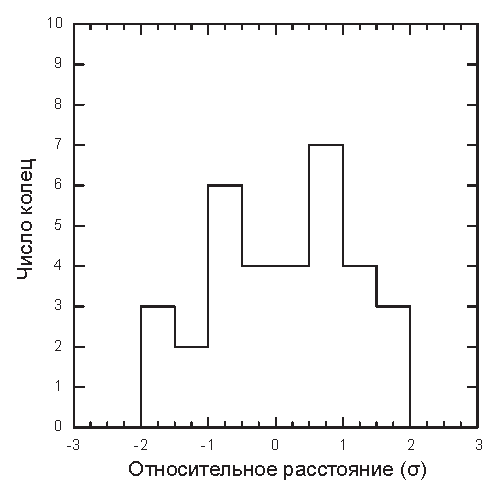
\includegraphics[width=0.5\textwidth]{dN_33_rel_offset}}
    \caption[Распределение расстояний от центра кольца до точного положения источника]
    {Распределение расстояний от точных позиций GRB до центральных линий 33-х колец, 
    полученных с использованием  KW и околоземного КА (или INTEGRAL).
    }
 \label{img:dN_33_rel_offset}  
\end{figure}

\FloatBarrier
\subsection{Дополнительные ограничения локализаций}
Помимо триангуляционных колец, было получено ещё несколько типов локализационной информации. 
Они включают: диапазон эклиптических широт, автономные локализации, полученные 
\textit{CGRO}-BATSE, \textit{BeppoSAX}-GRBM и \textit{Fermi}-GBM, а также области 
затенённые Землёй или Марсом (\textit{MESSENGER} находится на вытянутой орбите вокруг Меркурия, из-за этого, 
затенения Меркурием редки). Эта дополнительная информация помогает ограничить 
положение источника, полученное триангуляционным методом, например, 
выбрать одну из областей локализации или исключить часть кольца.

\subsubsection{Эклиптические широты}
Эклиптические широты всплесков вычисляются на основе отношения скоростей счёта
в двух детекторах KW, измеренных в режиме фон с разрешением 1.472 или 2.944~c. Ось
детектора S2 направлена в северный полюс эклиптики, а ось детектора S1~--- в южный.
Помимо статистической ошибки, получаемая эклиптическая широта имеет систематическую 
ошибку, связанную, помимо прочего, с переменными рентгеновскими источниками,
затенениями другими инструментами на борту стабилизированного вращением КА~\textit{Wind}.
Ошибки полученных значений были взяты на уровне 95\%.

Диапазон эклиптических широт, а именно, наилучшая оценка $b$, верхний и нижний
пределы $b_{\rmn{min}}$, $b_{\rmn{max}}$, можно рассматривать как кольцо с центром в северном или южном
полюсе эклиптики с углом раствора $\theta = 90^\circ - |b|$ и полуширинами 
$d_{-}(\theta) = b_{\rmn{min}} - b$ и $d_{+}(\theta) = b_{\rmn{max}} - b$.

\subsubsection{Затенения планетами}
Затенения планетой задаётся прямым восхождением и склонением центра планеты и её
радиусом. При наблюдении всплеска на околоземном или околомарсианском КА планета
затеняет до $\approx 3.7$~ср~неба. Положение источника должно быть вне этой 
затенённой части неба.

Разрешенная часть неба может быть представлена как вырожденное кольцо с центром
в направлении, противоположном центру планеты с углом раскрытия $\theta =0$ и 
полу ширинами $d_{-}(\theta) = 0$ и $d_{+}(\theta)= \arcsin(R_{\rmn{planet}}/R)$, 
где $R$~--- радиус орбиты КА (здесь мы пренебрегаем сплюснутостью планеты 
и поглощением излучения в её атмосфере.

\subsubsection{Автономные локализации}
Принцип автономной локализации всплесков с помощью системы детекторов с анизотропной 
чувствительностью был предложен в~\citep{Golenetskii_1974CosRe} и впервые реализован 
в системе Конус на КА Венера~11 и~12~\citep{Mazets_1981ApSS}. Схожие системы локализации 
с различным числом детекторов были установлены на KA \textit{CGRO} (BATSE), 
\textit{BeppoSAX} (GRBM) и \textit{Fermi} (GBM). Автономная локализация рассчитывается 
на основе соотношения скоростей счёта в детекторах. При этом на локализацию влияет 
альбедо Земли и поглощение излучения в конструкциях КА. Полученные локализации 
представляют собой плотность вероятности положения источника на небесной сфере. 
Локализации обычно имеют сложную форму и аппроксимируются кругом с центров в точке 
наиболее вероятного положения источника, радиус выбирается таким образом, 
чтобы площадь круга была равна соответствующей площади реальной области локализации 
для уровней значимости $1\sigma$ (BATSE, GBM) или 90\% (GRBM), с учётом только 
статистической неопределённости. Все локализации подвержены систематическим ошибкам 
не менее нескольких градусов.

Эти области также могут быть описаны вырожденным кольцом с центром в точке
наиболее вероятного положения источника, углом раскрытия $\theta =0$ и с ширинами 
$d_{-}(\theta) = 0$ и $d_{+}(\theta)= r$, где $r$~--- ошибка положения источника.

\section{Результаты локализации}
Информация по локализации 271 короткого всплеска Конус-Винд доступна на сайте 
ФТИ\footnote{\url{http://www.ioffe.ru/LEA/shortGRBs/Catalog2/Data/tables/}}.
Первая колонка содержит обозначение всплеска. Вторая колонка даёт 
число ограничений на локализацию всплеска (число строк с локализационной информацией 
для всплеска). Третья колонка содержит название источника локализации: 
КА1–КА2 (триангуляционное кольцо, полученное с использованием КА1 и КА2) или 
<<Ecl.Band>>\ (диапазон эклиптических широт), или <<Instrument>>\ (название инструмента, 
автономно локализовавшего всплеск), или <<Occ.sc>>\ (затенение планетой). 
Колонки (4)--(8) содержат прямые восхождения и склонения центров колец (J2000), 
угол раствора кольца $\theta$, и $3\sigma$ ошибки радиуса $d_{-}(\theta)$ и $d_{+}(\theta)$.

Затенения планетами даны только в случаях если они ограничивают локализацию. 
Диапазон эклиптических широт дан для всех всплесков. Также приведены все автономные 
локализации.

Локализации \textit{Swift}-BAT взяты из второго каталога \textit{Swift}-BAT, 
охватывающего период с 19~декабря 2004 по 21~декабря 2009~\citep{Sakamoto_2011ApJS}. 
Для более поздних всплесков локализации взяты из циркуляров GCN 
(\url{http://gcn.gsfc.nasa.gov/gcn3_archive.html}) с уточнённой локализацией BAT.

Локализация HETE-2 всплеска GRB~040924 (=GRB20040924\_T24735) взята из~\citep{Arimoto_2006GCN}.

Локализация IBIS/ISGRI всплеска GRB~070707 (=GRB20070707\_T58122) взята из~\citep{Gotz_2007GCN}.

Локализации BATSE взяты из каталога на сайте 
эксперимента\footnote{\url{http://www.batse.msfc.nasa.gov/batse/grb/catalog/current/}}, 
а также из каталога нетриггерных всплесков BATSE~\citep{Kommers_2000ApJ, Stern_2001ApJ}. 
Каталог~\citep{Stern_2001ApJ} содержит локализации всех восьми коротких всплесков Конус-Винд, 
зарегистрированных BATSE в режиме непрерывной записи, в каталоге~\citep{Kommers_2000ApJ} часть из них пропущена, 
приведённые локализации взяты исключительно из~\citep{Stern_2001ApJ}.

Локализации \textit{BeppoSAX} взяты как из каталога GRBM~\citep{Frontera_2009ApJS} 
так и из циркуляров IAU (\url{http://www.cbat.eps.harvard.edu/iauc/RecentIAUCs.html}) 
и GCN. 

Локализации GBM взяты из первого каталога \textit{Fermi}-GBM, охватывающего период с
12~июля 2008 по 11~июля 2010~\citep{Paciesas_2012ApJS}, циркуляров GCN или из последних 
версий соответствующих glg\_tcat*.fit файлов из архива GBM 
(\url{ftp://legacy.gsfc.nasa.gov/fermi/data/gbm/}).

\subsection{Пересечения колец}
Для всплесков, зарегистрированных тремя или более достаточно удалёнными друг от 
друга КА, может быть получена область локализации (бокс) в виде четырёхугольника 
или более сложной формы.

В общем случае пересечение двух колец, построенных с использованием дальнего КА,
даёт маленький бокс с площадью вплоть до одной квадратной угловой минуты.

Пересечение двух колец, полученных с использованием дальнего КА, Конус-Винд и
околоземного КА обычно даёт вытянутый бокс, который тем не менее имеет небольшую
площадь в несколько сотен квадратных угловых минут. В некоторых случаях пересечение кольца, полученного
с использованием дальнего КА, Конус-Винд и околоземного КА может дать бокс меньшей
площади, чем с использованием двух дальних КА.

Протяженные боксы были получены для всплесков, не зарегистрированных ни одним дальним КА, 
но зарегистрированные KW, \textit{INTEGRAL} (SPI-ACS) и одним иди более околоземным КА. 
В этих случаях бокс образуют кольцо KW--околоземный КА и
кольцо \textit{INTEGRAL}--околоземный~КА или кольцо KW--околоземный КА 
и кольцо KW--\textit{INTEGRAL}, пересекающиеся под достаточно острым углом.
Во всех случаях, когда КА используемые для триангуляции, практически лежат на
одной линии кольца пересекаются под очень острыми углами, образуя протяженный бокс.
Сумаарно было получено 162 бокса для коротких всплесков Конус-Винд: 27 для всплесков, 
зарегистрированных двумя дальними КА; 84 для всплесков, зарегистрированных одним 
дальним КА, и, по крайней мере, одним околоземным КА и 51 для всплесков, 
зарегистрированных KW, INTEGRAL и, по крайней мере, одним околоземным КА. В некоторых
случаях полученные области локализации представляют собой дуги (значительные части
колец).

\subsection{Сегменты}
Для всплесков, зарегистрированных только KW и другим КА или KW 
и одним или более околоземных КА, полученная локализация представляет часть кольца 
(наиболее узкого при детектировании несколькими околоземными КА), удовлетворяющая 
дополнительными ограничениями. Эти локализации представляют собой целое кольцо 
(если оно полностью находится внутри ограничений на эклиптическую широту и 
отсутствуют другие ограничения), или один или два сегмента кольца, образованные 
пересечением кольца и диапазоном эклиптических широт, и/или исключением затенённой 
планетой части кольца, или часть кольца, ограниченная локализацией BATSE (см. раздел~\ref{sec:KW_BATSE_cc}).
Описанный тип локализации имеют 114 всплесков: 20~--- всплески, зарегистрированные 
KW и одним дальним КА (из них 3 зарегистрированы одним околоземным КА в режиме 
непрерывной записи, но для них не было получено кольцо KW--околоземный КА) и 94 
всплеска были зарегистрированы только KW и одним или более околоземным КА.

\subsection{Полученные области локализации}
Окончательные области локализации для 254 коротких всплесков KW 
(в список не включены 17 точно локализованных всплесков) приведены на ресурсе 
\url{http://vizier.cfa.harvard.edu/vizier/ftp/cats/J/ApJS/207/38/table3.dat}.
Девять колонок таблицы содержат: 
(1) обозначение всплеска; (2) число областей локализации всплеска $N_{\rmn{r}}$ (1 или 2); 
(3) число углов у области локализации $N_{\rmn{c}}$, 
(4) тип области: <<B>>\ (бокс), <<LB>>\ (протяженный бокс: бокс с наибольшим размером $> 10^\circ$),
<<S>>\ (сегмент) или <<A>>\ (кольцо);
(5) площадь области (или сумма площадей в случае двух областей локализации); 
(6) наибольший размер области (наибольшее угловое расстояние между двумя точками границы области; 
для сегментов больших чем половина кольца приведён внешний диаметр кольца);
(7) название локализаций, формирующих область;
(8) прямое восхождение центра области, в первой строке, и прямое восхождение 
всех углов области в последующих $N_\rmn{c}$ строках и 
(9) склонения центра области, в первой строке, и склонение всех углов области в последующих
$N_\rmn{c}$ строках. В случае двух областей локализации дополнительно даны $N_{\rmn{c}} + 1$ строк: 
центр второй области и её углы. 
Таким образом, для таких всплесков дано $2(N_{\rmn{c}} + 1)$ строк. Все координаты даны на эпоху J2000.
В общем случае область локализации не может быть полностью описана четырёхугольником, 
для точного представления должна учитываться кривизна колец. Только в случаях, 
когда максимальный размер области не превышает нескольких градусов, 
область может описываться только четырьмя углами. В других случаях, когда область переставляет
собой длинную дугу или сегмент кольца приведённые центр и углы области предназначены
для приблизительного указания положения области на небе. Рисунки, иллюстрирующие
IPN локализации (все вычисленные кольца и полученные области) можно найти на сайте
ФТИ им.~А.~Ф.~Иоффе (\url{http://www.ioffe.ru/LEA/ShortGRBs_IPN/}).

Распределение площадей полученных областей локализаций приведено на Рис.~\ref{img:dN_256_areas}.
Для всплесков, зарегистрированных дальними КА, площади находятся в диапазоне от 
$2.40 \times 10^{-4}$~deg$^2$ 0.86~arcmin$^2$) до 142~deg$^2$ со средним 3.49~deg$^2$ 
и геометрическим средним 0.141~deg$^2$. Для всплесков, не зарегистрированных дальними КА, 
площади находятся в диапазоне от 0.210~deg$^2$ до 4420~deg$^2$ со средним 242~deg$^2$
и геометрическим средним 46.2~deg$^2$.

\begin{figure}[h]
    \center{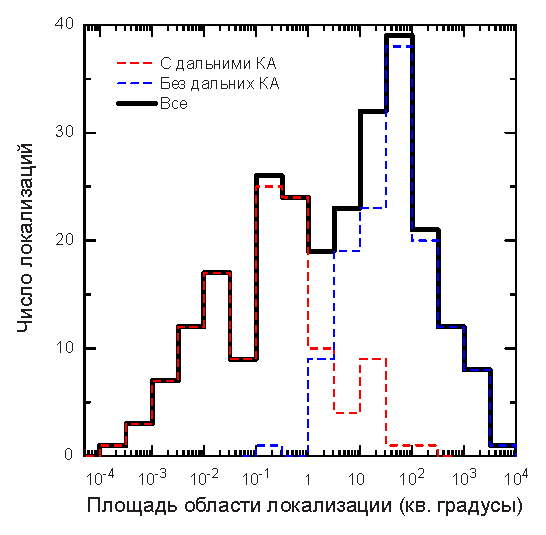
\includegraphics[width=0.5\textwidth]{dN_256_areas}}
    \caption[Распределение площадей 256 областей локализации]
    {Распределение площадей областей локализации для 123 коротких всплесков Конус-Винд
    наблюдавшихся, по крайней мере, одним дальним КА (красная пунктирная линия) и 
    131 всплеска, не наблюдавшегося ни одним дальним КА (синяя пунктирная линия). 
    Суммарное распределение 254 всплесков обозначено непрерывной линией 
    (17 точно локализованных всплесков не использовались при построении распределения).
    }
 \label{img:dN_256_areas}  
\end{figure}
\FloatBarrier
\section{Обсуждение особых событий}
GRB~051103 (=GRB20051103\_T33943) может являться гигантской вспышкой мягкого 
гамма-репитера (SGR) в близкой группе взаимодействующих галактик M81, что было 
предложено в работе~\citep{Frederiks_2007AstL}. Итоговая область локализации 
этого события совместно с дальнейшим исследованием предложенной природы этого 
события приведено в~\citep{Hurley_2010MNRAS}. В работе~\citep{Ofek_2006ApJ} 
приведены выводы, сделанные на основе оптических и радио наблюдений, последовавших 
за детектированием всплеска в гамма-диапазоне. В работе~\citep{Abadie_2012ApJ} обсуждается
не детектирование гравитационных волн во время этого события.

GRB~070201 (=GRB20070201\_T55390) вероятно является гигантской вспышкой SGR
в туманности Андромеды~\citep{Mazets_2008ApJ}. В работе~\citep{Abbott_2008ApJ} 
обсуждаются результаты недетектирования гравитационных волн от этого события 
и в~\citep{Ofek_2008ApJ} обсуждается недетектирование оптического послесвечения 
и периодического рентгеновского источника.

Поиск других кандидатов в гигантские вспышки SGR на основе полученных локализаций 
приведён в следующей главе.

GRB~000420 (=GRB20000420\_T42271) на основании кольца KW--\textit{NEAR} 
был отнесён в работе~\citep{Ofek_2007ApJ} к кандидатам в гигантские вспышки SGR 
в близкой галактике M74 (NGC~628). Положение этой галактики находится 
вне кольца KW--\textit{BeppoSAX}, таким образом исключая возможность 
происхождения этого всплеска в M74 (см.~Рис.~\ref{img:GRB000420_loc}).

\begin{figure}[h]
    \center{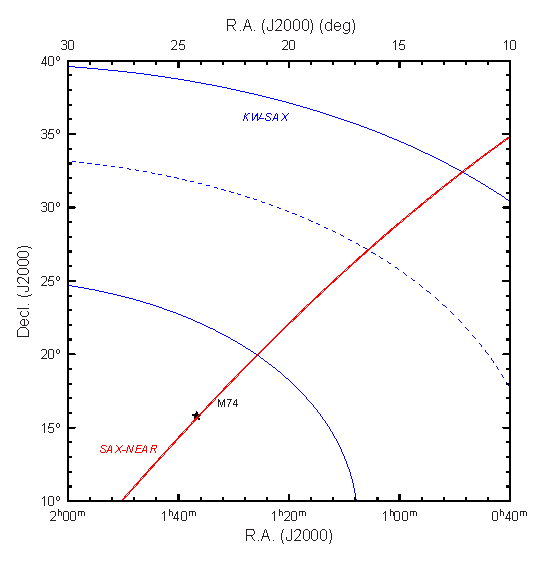
\includegraphics[width=0.5\textwidth]{GRB000420_loc}}
    \caption[Локализация всплеска GRB~000420]
    {IPN локализация GRB 000420 (= GRB20000420\_T42714).
    Узкое кольцо SAX-NEAR, шириной $1\farcm7$, проходит через близкую галактику M74,
    в то время как галактика лежит далеко за пределами широкого $3\sigma$ кольца KW-SAX.
    }
 \label{img:GRB000420_loc}  
\end{figure}

GRB~990405 (=GRB19990405\_T30059) изначально был классифицирован как всплеск
от SGR~1900+14 так как узкое кольцо \textit{BeppoSAX}--\textit{Ulysses} 
(с $3\sigma$ полушириной $0\fdg035$) проходило через положение 
этого SGR. Полученное кольцо KW--\textit{BeppoSAX} (с $3\sigma$ полушириной
$6\fdg4$) также согласуется положением этого SGR. Но этот всплеск 
существенно жестче, чем два необычно жестких всплеска из SGR~1900+14: 
981022 и 991001~\citep{Woods_1999ApJ}, делая ассоциацию этого всплеска 
с SGR~1900+14 сомнительной.
\FloatBarrier

\section{IPN локализация всплесков, наблюдаемых iPTF}
Короткие гамма-всплески являются наиболее вероятными источниками гравитационных
волн. Для детектирования грав. волн созданы детекторы  Advanced~LIGO~\citep{Harry_2010CQGra} 
и Virgo~\citep{Accadia_2012JInst}, которые будут способны зарегистрировать сигнал от слияния
двух нейтронных звёзд на расстоянии в несколько сотен мегапарсек.
Область локализации источников гравитационных волн, в случае использования 
трёх детекторов может иметь размер до $\approx 300$~deg$^2$~\citep{Singer_2015PhDT}.

Основным инструментом для поиска оптических транзиентов, связанных с источниками 
гравитационных волн, в настоящее время является телескоп P48, входящий в состав 
системы телескопов для поиска транзиетов Паломарской обсерватории
(iPTF, \textit{Intermediate Palomar Transient Factory}~\citep{Rau_2009PASP}). 
Телескоп имеет диаметр $\approx 1.2$~м, поле зрения 7 квадратных градусов и 
чувствительность на уровне $5\sigma$ в фильтре $R$ (570--730~нм) $\approx 21$ зв.~величина за минутную экспозицию.
%Инструмент может выполнять съёмку заданной области на небе.
Для проверки возможностей инструмента проводится кампания по наблюдению локализаций
гамма-всплесков, зарегистрированных \textit{Fermi}-GBM и IPN.

Длинный гамма-всплеск GRB~120716A был зарегистрирован  \textit{Fermi}-GBM, Konus-\textit{Wind}, 
\textit{INTEGRAL}-SPI-ACS, \textit{Suzaku}-WAM и \textit{MESSENGER}-GRNS,
пощадь полученной локализации  составила $\approx 2$ квадратных градуса~\citep{Hurley_2012GCN13487}.
Оптическое послесвечение всплеска было обнаружено iPTF 
через $\sim 1.5$ дня~\citep{Cenko_2012GCN13489}, на расстоянии 3 угловые минуты от центра локализации.
% возможно стоит подробней написать про этот всплеск - длинный с коротким прекурсором.

За период с 2013 по 2014~гг. iPTF наблюдала локализации 35 гамма-всплесков, зарегистрированных GBM,
для восьми было обнаружено послесвечение. Из них, в четрёх случаях отбор кандидатов
был упрощён благодаря IPN локализации.


\section{Заключение}
В этой главе представлено продолжение серии каталогов локализаций гамма-всплесков 
триангуляционным методом с использованием КА сети IPN. Список предшествующих каталогов 
приведён в таблице~\ref{tab:IPN_cat}.

Полученные локализации могут быть использованы для большого круга задач, включающего: 
поиск гравитационных волн и нейтрино от слияния компактных объектов, 
поиск гамма-квантов сверхвысоких энергий из источников всплесков и поиск гигантских 
вспышек SGR в ближайших галактиках.

\begin{table} [h]
 \centering
 \caption{Каталоги IPN локализаций гамма-всплесков}\label{tab:IPN_cat}
\scriptsize
  \begin{center}
  \begin{tabular}{ccc}
  \hline
  \hline
  Период покрытия, годы & Число всплесков & Описание \\
  \hline
1990--1992 &16 &\textit{Ulysses}, \textit{Pioner Venus Orbiter}, WATCH, SIGMA, PHEBUS GRBs~\citep{Hurley_2000ApJ} \\
1990--1994 &56 &\textit{GRANAT}-WATCH supplement~\citep{Hurley_2000ApJS_WATCH} \\
1991--1992 &37 &\textit{Pioner Venus Orbiter}, \textit{CGRO}, \textit{Ulysses} GRBs~\citep{Laros_1998ApJS}\\
1991--1994 &218 &BATSE 3B supplement~\citep{Hurley_1999ApJSa}\\
1991--2000 &211 &BATSE untriggered GRBs supplement~\citep{Hurley_2005ApJS_BATSE_untrig}\\
1992--1993 &9 &\textit{Mars Observer} GRBs~\citep{Laros_1997ApJS}\\
1994--1996 &147 &BATSE 4Br supplement~\citep{Hurley_1999ApJS_BATSE_4Br}\\
1994--2010 &271 &короткие гамма-всплески Конус-Винд (эта работа)\\
1996--2000 &343 &BATSE 5B supplement~\citep{Hurley_2011ApJS_BATSE_5B}\\
1996--2002 &475 &\textit{BeppoSAX} supplement~\citep{Hurley_2010ApJS_BeppoSAX}\\
2000--2006 &226 &HETE-2 supplement~\citep{Hurley_2011ApJS_HETE2}\\
2008--2010 &146 &\textit{Fermi}-GBM supplement~\citep{Hurley_2013ApJS_GBM}\\
  \hline
  \hline
  \end{tabular}
  \end{center}
\end{table}

\FloatBarrier

В главе получены следующие результаты:
\begin{enumerate}
\item В главе получена наиболее полная локализационная информация для 271 короткого 
гамма-всплеска Конус-Винд. Для 254 всплесков были получены области локализации и 
для 17 всплесков с точно известной локализацией, полученной инструментами с 
возможностью построения изображений в жестком рентгеновском диапазоне, триангуляционные
кольца получены для проверки методики.

Суммарно было получено 517 триангуляционных колец, включая 150 колец с использованием 
дальних КА. Показано, что для многих коротких всплесков триангуляции 
KW--околоземные~КА (или \textit{INTEGRAL}) дают достаточно узкое кольцо 
с полушириной сравнимой или меньше чем при использовании дальних КА. Таким образом, 
даже в случае детек-тирования всплеска только одним дальним КА (и одним и более 
околоземным КА) можно получить область локализации с площадью несколько 
сотен квадратных угловых минут. Для всплесков, зарегистрированных только KW, 
\textit{INTEGRAL} (SPI-ACS) и одним или более околоземным КА, получаются 
протяженные области локализации.

\item С использованием описанной методики были получены локализации 146 гамма-всплесков,
зарегистрированных \textit{Fermi}~(GBM) за период с 12 июля 2008~г. по 11 июля 2010~г.
На основании этих локализаций была определена систематическая ошибка $\approx 6^\circ$
для автономных локализаций GBM. Было установлено, что IPN локализации 
существенно уменьшению площади области локализации GBM, до 180~раз.  

\item Описанная методика была успешно применена для подтверждения оптических послесвечений,
зарегистрированных системой телескопов для поиска транзиетов Паломарской обсерватории.
\end{enumerate}

По материалам Главы~\ref{IPN_catalog} на защиту выносится следующее положение:
\begin{itemize}
\item Каталог локализаций коротких гамма-всплесков, зарегистрированных в эксперименте
    Конус-Винд с 1994~г. по 2010~г.
\end{itemize}

Результаты, описанные в главе, отражены в следующих публикациях:
\begin{enumerate}
\item V.~D. Pal'shin, K. Hurley, D.~S. Svinkin et al., Interplanetary Network Localizations of
Konus Short Gamma-Ray Bursts // Astrophys.~J.~Suppl. 2013. Vol.~207. id~38;
\item K. Hurley, (D.~S. Svinkin) et al., The Interplanetary Network Supplement to 
the Fermi GBM Catalog of Cosmic Gamma-Ray Bursts // Astrophys.~J.~Suppl. 2013. Vol.~207. id~39;
\item Leo P. Singer, (D.~Svinkin), et al., The Needle in the 100 deg$^2$ Haystack: 
Uncovering Afterglows of Fermi GRBs with the Palomar Transient Factory // 
Astrophys.~J. 2015. Vol.~806.
\end{enumerate}


\clearpage